\documentclass[12pt]{report}
\usepackage{graphicx}
\usepackage{array}
\usepackage{tabularx}
\usepackage{amsmath}
\usepackage{hyperref}
\usepackage{geometry}
\usepackage{fontspec} % For custom fonts
\usepackage{xcolor}
\usepackage{float}
\usepackage{titling}
\usepackage{tikz}
\usepackage{fancyhdr} % For custom headers/footers
\usepackage{tocbibind} % To include TOC, LOF, LOT in TOC
\setmainfont{Times New Roman} % Set the main font to Times New Roman
\geometry{a4paper, margin=1in}
\usepackage{setspace}
\onehalfspacing 
\usepackage{titlesec}
\usepackage{fancyhdr}
\pagestyle{fancy}
\fancyhf{} % Clear all header and footer fields
\fancyfoot[C]{\thepage} % Place the page number in the center of the footer
\renewcommand{\headrulewidth}{0pt}  % Removes the line in the header
\renewcommand{\footrulewidth}{0pt}  % Removes the line in the footer
\hypersetup{
   colorlinks=true,
  linkcolor=black,   % Set link color to black
  filecolor=magenta, 
  urlcolor=cyan,
  pdfborder={0 0 0} 
}
\renewcommand{\contentsname}{SOMMAIRE GENERAL} 
\renewcommand{\listtablename}{LISTE DES TABLEAUX}
\renewcommand{\listfigurename}{LISTE DES FIGURES}

\titleformat{\chapter}[display]
    {\normalfont\large\bfseries\centering}
    {PARTIE \Roman{chapter}~.}
   {20pt}
    {\Large}

\titleformat{\section}
    {\normalfont\bfseries} 
    {\thesection}
    {1em}
    {}
	
\begin{document}	
			 \pretitle{
				\begin{tikzpicture}[remember picture, overlay]
			   		\node[anchor=north west, xshift=1.5cm, yshift=-1cm] at (current page.north west) {
        						\includegraphics[width=2.5cm]{image1.png}
					};
    					\node[anchor=north west, xshift=4cm, yshift=-1cm] at (current page.north west) {
        						\includegraphics[width=2.3cm]{image2.png}
					};
					\node[anchor=north east, xshift=-1.5cm, yshift=-1cm] at (current page.north east) {
        						
\includegraphics[width=5cm]{image3.png}
					};
				\end{tikzpicture}
				\begin{center}
					\textbf{\large UNIVERSITE DE FIANARANTSOA ECOLE NATIONALE D'INFORMATIQUE \\[0.5cm] MEMOIRE DE FIN D'ETUDES POUR L'OBTENTION DU DIPLOME DE MASTER PROFESSIONNELLE}
					\\[0.5cm]
							\textbf{\underline{Mention:}} Informatique \\	
							\textbf{\underline{Parcours:}} Informatique générale\\
							\textbf{\textit{Intitulé}}				\end{center}
				\begin{center}\large\bfseries
			}
			\preauthor{\begin{flushleft}\fontsize{12} \lineskip Présenté le 01 février 2023 }
			\postauthor{\end{flushleft} \textbf{Membres du Jury:} 
			 \begin{itemize}
			    \item \textbf{Président:} Monsieur RALAIVAO Jean Christian, Assistant d'Enseignement Supérieur et de Recherche;
			    \item \textbf{Examinateur:} Monsieur RALAIVAO Jean Christian, Assistant d'Enseignement Supérieur et de Recherche;
			    \item \textbf{Rapporteurs:} \begin{itemize}
       									 \item Monsieur RALAIVAO Jean Christian, Assistant d'Enseignement Supérieur et de Recherche;
       									 \item Monsieur RALAIVAO Jean Christian, Assistant d'Enseignement Supérieur et de Recherche.
    								\end{itemize}
			\end{itemize} }
			\predate{\begin{flushright} Année Universitaire: }
			\postdate{\end{flushright}}
			\title{
				\color{blue}
				\setlength{\fboxsep}{10pt} 
				\fbox{
					\begin{minipage}{0.95\textwidth}
						\begin{center}
							CONCEPTION ET REALISATION  D'UNE APPLICATION WEB  DE RESERVATION DE VOYAGE
						\end{center}
					  \end{minipage}
				}
			}
			\author{\textbf{Par:} Monsieur ANDRIAMIORA Ainamalala Lucky}
			\date{2024-2025}
			\maketitle
			
			\newpage
			\thispagestyle{empty}
			\mbox{}

			\newpage
			\pagenumbering{roman}
			\renewcommand{\thepage}{\Roman{page}} % Ensure uppercase Roman numerals
			\setcounter{page}{1}
			\chapter*{CURRICULUM VITAE}
			\addcontentsline{toc}{chapter}{CURRICULUM VITAE}	
			\begin{minipage}{0.6\textwidth}
				\textbf{Nom:} ANDRIAMIORA\\
				\textbf{Prenom:} Ainamalala Lucky\\
				\textbf{Numéro:} +261 34 33 513 61\\
				\textbf{Addresse:} IIG20 E Ambatomaro, Antananarivo\\
				\textbf{E-mail:} luckyainamalalalucky@gmail.com\\
				\textbf{Date et lieu de naissance:} 30 décembre 1999 à Antsirabe
			\end{minipage}
			\hfill
			\begin{minipage}{0.3\textwidth}
				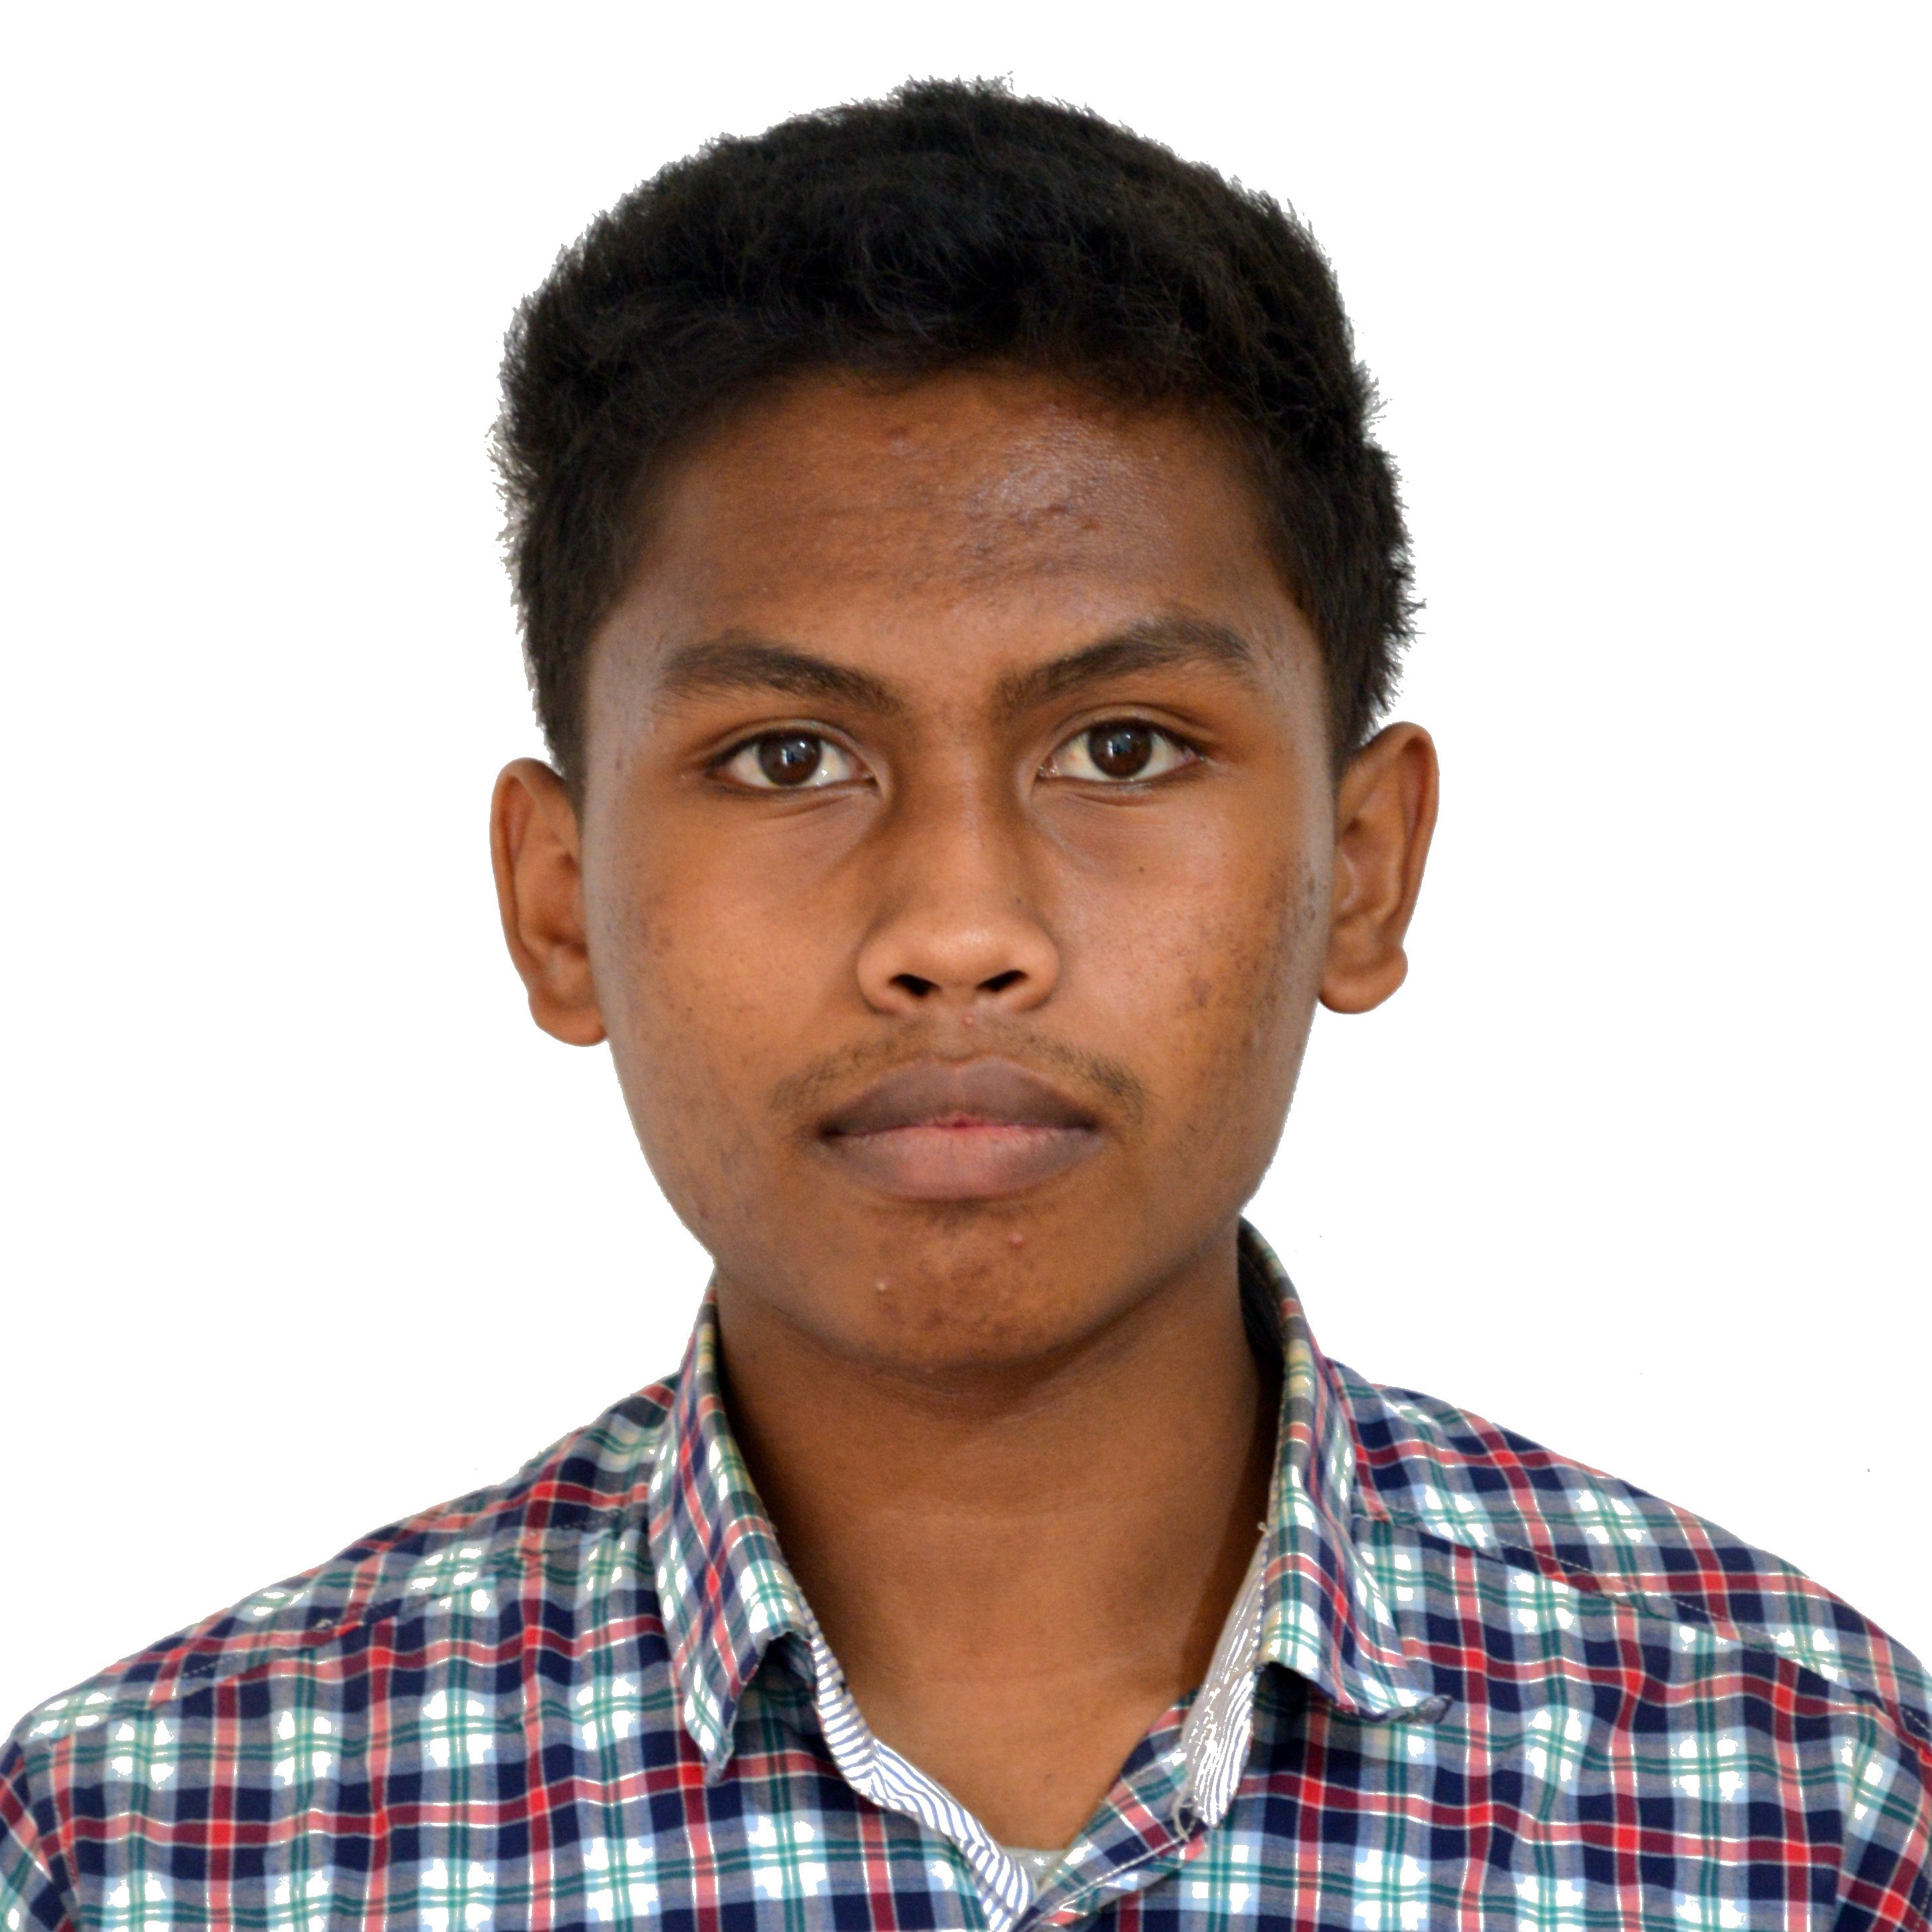
\includegraphics[width=3.5cm, height=3.5cm]{mypic.jpg}	
			\end{minipage}
			\section*{FORMATIONS ET DIPLOME}
			\begin{minipage}{\textwidth}
				\textbf{2024-2025:} Deuxième année de formation en Master professionnelle à l’École Nationale d'Informatique, Université de Fianarantsoa, parcours : Informatique générale.\\[0.5cm]
				\textbf{2023-2024:} Première année de formation en Master professionnelle à l’École Nationale d'Informatique, Université de Fianarantsoa, parcours : Informatique générale.\\[0.5cm]
				\textbf{2022-2023:} Obtention du diplôme de Licence professionnelle mention Bien à l’École Nationale d'Informatique, Université de Fianarantsoa, parcours : Informatique générale.\\[0.5cm]
				\textbf{2021-2022:} Deuxième année de formation en Licence professionnelle à l’École Nationale d'Informatique, Université de Fianarantsoa, parcours : Informatique générale.\\[0.5cm]
				\textbf{2020-2021:} Première année de formation en Licence professionnelle à l’École Nationale d'Informatique, Université de Fianarantsoa, parcours : Informatique générale.\\[0.5cm]
				\textbf{2019-2020:} Obtention du diplôme de Baccalauréat série D mention assez-bien au Lycée André Résampa Antsirabe.
			\end{minipage}
			\section*{STAGES ET EXPERIENCES PROFESSIONNELLES}
				\begin{minipage}{\textwidth}
       					 \textbf{11 juin 2024 au 4 novembre 2024:} Stage auprès de Nexitia technologies.
						\begin{itemize}
							\item Thème du stage: Application web Handeha voyage;
							\item Langages et outils: Java, spring boot, JavaScript, next js, Katappult, H2, UML.						
						\end{itemize}
       					 \textbf{Octobre 2023:} Projet à l’École Nationale d'Informatique.
						\begin{itemize}
							\item Thème du stage: Module de securité pour application spring boot et angular;
							\item Langages et outils: Java, spring boot, Angular, TypeScript, PostgreSQL, UML.						
						\end{itemize}       					 
					\textbf{19 octobre 2022 au 16 janvier 2023:} Stage auprès de la Paositra malagasy.
						\begin{itemize}
							\item Thème du stage: Application web pour la gestion des change;
							\item Langages et outils: Java, spring boot, Angular, TypeScript, PostgreSQL, UML.								
						\end{itemize}
					\textbf{Septembre 2022:} Projet à l’École Nationale d'Informatique.
						\begin{itemize}
							\item Thème du stage: Création d'une application mobile de gestion de cotisation de groupe;
							\item Langages et outils: Java, Android Studio.								
						\end{itemize}
					\textbf{8 mars 2021 au 7 juillet 2021:} Stage auprès du Ministère de l’Économie et de la Finance.
						\begin{itemize}
							\item Thème du stage: Application web pour la gestion des dossier du personnels de la Direction du Système d'Information;
							\item Langages et outils: Java, spring boot, Angular, TypeScript, PostgreSQL, UML.								
						\end{itemize} 
					\textbf{Avril 2021:} Projet à l’École Nationale d'Informatique.
						\begin{itemize}
							\item Thème du stage: Réalisation d’une application desktop de Gestion des heures complémentaires;
							\item Langages et outils: Php, MySQL, Ajax.								
						\end{itemize} 
					\textbf{Août 2020:} Projet à l’École Nationale d'Informatique.
						\begin{itemize}
							\item Thème du stage: Création d'une application desktop de gestion de stock;
							\item Langages et outils: C++, Qt Creator.								
						\end{itemize} 
   				\end{minipage}		
			\section*{CONNAISSANCES EN INFORMATIQUE}
			\begin{minipage}{\textwidth}
				\begin{itemize}
					\item \textbf{Systèmes d'exploitation:} Microsoft Windows, Linux;
					\item \textbf{Langages de Programmation:} Java, JavaScript, TypeScript, Python , C/C++;
					\item \textbf{Développement Web:} HTML5, CSS3, Tailwind CSS, React.js, Next.js, Angular, Node.js, Express.js;
					\item \textbf{Développement Backend:} Spring Framework, Node.js, Express.js;
					\item \textbf{Compétences en bases de données:} SQL, PostgreSQL, MySQL;
					\item \textbf{Outils de Gestion de Versions:} Git, GitHub, GitLab; 	
					\item \textbf{Outils DevOps:} Docker, Kubernetes, Jenkins, Ansible;
					\item \textbf{Outils de virtualisation:} Docker, VirtualBox, VMware, Vagrant; 	
					\item \textbf{Outils de tests et Assurance Qualité:} Jest, JUnit;
					\item \textbf{Outils et Méthodologies de Conception et Gestion de Projets Logiciels:} UML, Méthodologie Agile, 2TUP, MERISE, GRASP;
					\item \textbf{Outils de Documentation et de Préparation de Contenu:} LaTeX/TeX.	
				\end{itemize}

   			\end{minipage}		
			\section*{CONNAISSANCES LINGUISTIQUE}
			\begin{minipage}{\textwidth}
				\begin{center}
					\begin{tabularx}{\textwidth}{|c|X|X|X|X|}
						\hline
						\textbf{LANGUE} & \textbf{COMPREHENSION} & \textbf{LECTURE} & \textbf{PARLE} & \textbf{ECRIT}\\
						\hline
						Anglais & Bien & Bien & Assez-bien & Bien \\
						\hline
						Français & Bien & Bien & Bien & Bien\\
						\hline
					\end{tabularx}
				\end{center}
			\end{minipage}
			\section*{LOISIR ET CENTRES D'INTERET}
			\begin{minipage}{\textwidth}
				\begin{itemize}
					\item Musique;
					\item Podcast;
					\item Documentaires;
					\item Anime;
					\item Jeux video;
					\item	Lecture.
				\end{itemize}
			\end{minipage}	
			\chapter*{REMERCIEMENTS}
			\addcontentsline{toc}{chapter}{REMERCIEMENTS}	
			\begin{minipage}{\textwidth}
				\hspace{15pt} Avant toute chose, je tiens à remercier Dieu tout puissant et miséricordieux, qui m'a donné la force et la patience d'accomplir ce modeste travail.\\[0.5cm]
				Mes remerciements s’étendent également à :
				\begin{itemize}
					\item Monsieur HAJALALAINA Aimé Richard, Docteur HDR, Président de l'Université de Fianarantsoa, pour tout ce qu'il entreprend à l'Université;
					\item Monsieur MAHATODY Thomas, Docteur HDR, Directeur de l’École Nationale d'Informatique, qui nous à donné l'opportunité d'aller en stage pour ainsi permettre d’accroître nos compétences;
					\item Monsieur RANARISON Richard, Directeur Général de la Paositra Malagasy, pour son accueil et la confiance qu'il à accordée depuis mon arrivée dans l’établissement;
					\item Monsieur RATIARSON Venot, Maître de Conférences, mon encadreur pédagogique, pour ses conseils et échanges tout au long du stage;
					\item Madame RANDRIAMIHARISOA Rollande, mon encadreur professionnelle, qui m'a toujours guidée lors de la réalisation du projet;
					\item Monsieur RALAIVAO Jean Christian, Assistant d'Enseignement Supérieur et de Recherche,d’avoir accepté de présider la soutenance;
				 	\item Monsieur DIMBISOA William Germain, Docteur en Informatique, d'avoir accepté d'examiner mon présent travail;
					\item Toutes les personnels de la Paositra Malagasy, pour leurs accueils;
					\item Toutes les enseignants et les personnels de l’École Nationale d'Informatique qui se sont acharné à nous former durant l'année universitaire;
					\item Ma famille pour son soutien, que se soit moral, matériel ou financier.
				\end{itemize}
			\end{minipage}
			\newpage
			\tableofcontents
			\newpage
			\chapter*{NOMENCLATURE}
			\addcontentsline{toc}{chapter}{NOMENCLATURE}	
			\newpage
			\listoftables
			\newpage
			\listoffigures
			\newpage
			\newpage
			\pagenumbering{arabic}
			\setcounter{page}{1}
			\chapter*{INTRODUCTION GÉNÉRALE}
			\addcontentsline{toc}{chapter}{INTRODUCTION GÉNÉRALE}
			\begin{minipage}{\textwidth}
				\hspace{15pt} Avec sa biodiversité unique et sa richesse culturelle, Madagascar est une destination touristique de choix. Cependant, avec la demande pour des expériences de voyage personnalisées et accessibles en ligne en constante croissance, de nombreux opérateurs touristiques luttent pour obtenir la visibilité et les moyens nécessaires pour promouvoir efficacement leurs offres.\\

				\hspace{15pt} Malgré l'essor des plateformes de réservation en ligne, il demeure un besoin urgent d'une solution centralisée pour permettre aux opérateurs touristiques malgaches de partager leurs offres et aux voyageurs de réserver facilement leurs circuits ou séjours.\\

				\hspace{15pt} L'objectif de ce mémoire est de développer et de présenter "Handeha Voyage", une application web qui  facilite la mise en ligne des offres de circuits et de séjours par les opérateurs touristiques, simplifie le processus de réservation pour les utilisateurs et améliore la visibilité des opérateurs touristiques. Cette étude propose une solution novatrice qui répond directement aux défis rencontrés par les opérateurs touristiques et les voyageurs à Madagascar. En effet, l'application "Handeha Voyage" ne se contente pas de faciliter la réservation des voyages; elle redéfinit fondamentalement la manière dont les services touristiques sont présentés et consommés.\\

				\hspace{15pt} Ce mémoire abordera le processus de conception, de développement et de mise en œuvre de l'application "Handeha Voyage". Nous utiliserons des méthodes de conception et de modélisation adaptées, ainsi que des langages de programmation et frameworks appropriés, sans oublier un système de gestion de base de données solide. Tout cela sera orchestré selon une méthodologie de gestion de projet bien définie pour assurer une organisation optimale. Les limitations incluent le temps limité pour le développement complet de certaines fonctionnalités avancées, l'accès limité aux données et la difficulté à recueillir des retours d'expérience durant le développement.\\

				\hspace{15pt} Notre plan se subdivise en trois parties: dans un premier temps la présentation de l’École Nationale d'Informatique (ENI) suivie de celle de Nexitia Technology. Dans la deuxième partie, nous aborderons les analyses et la conception du projet. Enfin, la troisième partie portera sur la réalisation du projet avec les différents moyens et outils utilisés.
			\end{minipage}
			\newpage
			\chapter{PRESENTATION}
\end{document}